\documentclass[a4paper,12pt]{jsreport}
\usepackage{bm}
\usepackage[dvipdfmx]{graphicx}
\usepackage{ascmac}

\title{ミリ波を用いた地中埋設物の位置と形状の推定}
\author{廣瀬夏秋研究室\\
学籍番号03-210499 高原陽太}


\begin{document}
\maketitle
\tableofcontents

\chapter{はじめに}

最初はイントロ的なことを書く。
\section{現状と問題点}

最近の現状と問題点とか。

\section{解決策の提案}

こうしたらいい,とか。

\section{数式の書き方}

アインシュタイン方程式は以下の通りである。
% \begin{equation}
% R_{\mu\nu} - \frac{1}{2} g_{\mu\nu} R =
% \frac{8\pi G}{c^2} T_{\mu\nu}
% \end{equation}

\chapter{原理と提案手法}

この辺から本番。

\section{地中レーダーの原理}
 地中レーダーは電磁波の地下物体からの
反射を利用した地下計測手法である。電磁波パルスを地表に置かれた送信アンテナ
から地中に放射し、受信アンテナで受信する。地中を伝搬する電磁波は、土壌中に
誘電率が異なる物質が存在すると反射を起こす性質があり、そのため埋設物の材料物質
と誘電率の違いを利用して埋設物の存在を検知することが可能となっている。この反射の様子から
埋設物が埋まっている深度を計測する。
\\ 地中では電磁波速度は導電率、誘電率、透磁率によって決まる。しかしGPRでは1MHzより高い
周波数領域で計測が行われるため、地下媒質の電気的性質は比誘電率$\varepsilon$にのみ左右される。
この時の地中伝搬速度$v$は

\begin{equation}
  v =
  \frac{c}{\sqrt{\varepsilon}} 
  \end{equation}

と書ける。


そして地中の伝搬速度が分かりさえすれば、送信電波が反射波として戻ってくる時間
$\tau$を計測することで図\ref{地中レーダーの様子}のように反射体の深度$d$は次式で導出できる。
\begin{equation}
  d=
  \frac{v \tau}{2} 
  \end{equation}
  
また同様に反射波の振幅も誘電率によって推定できる。図\ref{地中レーダーの様子}のように
誘電率の異なる二層媒質構造の場合について考える。この時上層から入射する電波は境界面で反射を受け
、振幅比$\Gamma$の反射波が発生する。

\begin{figure}[h]
  \begin{center}
   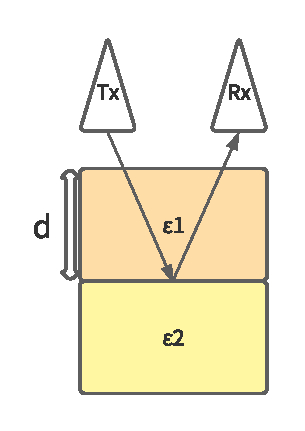
\includegraphics[width=7cm]{./image/radar.pdf}
   
  \caption{地中レーダーの様子}\label{地中レーダーの様子}
  \end{center}
  \end{figure}

反射係数$\Gamma$は境界面で以下のように与えられる。
\begin{equation}
  \Gamma=
  \frac{\sqrt{\varepsilon_{1}}-\sqrt{\varepsilon_{2}}}{\sqrt{\varepsilon_{1}}+\sqrt{\varepsilon_{2}}} 
\label{gamma}  
\end{equation}


式(\ref{gamma})は反射係数が二つの媒質の誘電率のみによって決まることを示している。
\\ これらの情報を測定することで埋設物の位置と材質を推定するのである。

\section{偏波}
 偏波とは図\ref{偏波のイメージ}のように電界と磁界が直行しながら伝搬する波である。偏波を用い、目標物に
照射することで目標物に関する情報を多々得ることができるため、GPRにも用いられている。単に埋設物の反射電力だけで
なく位相も反射によって変わるため、その情報も利用することができるという利点を持つ。
\\ 特に埋設物がパイプなどの線状物体である時に偏波の状態を観測することは重要になる。というのも電磁波の偏波方向と
線状物体の方向が一致するとき、大きな反射が起こるのに対して、偏波方向が線状物体と直行すると反射が非常に小さくなってしま
うからである。ゆえに受信した偏波の状態からパイプなどの物体の向きや形状も推定することが可能なのである。
\begin{figure}[h]
  \begin{center}
   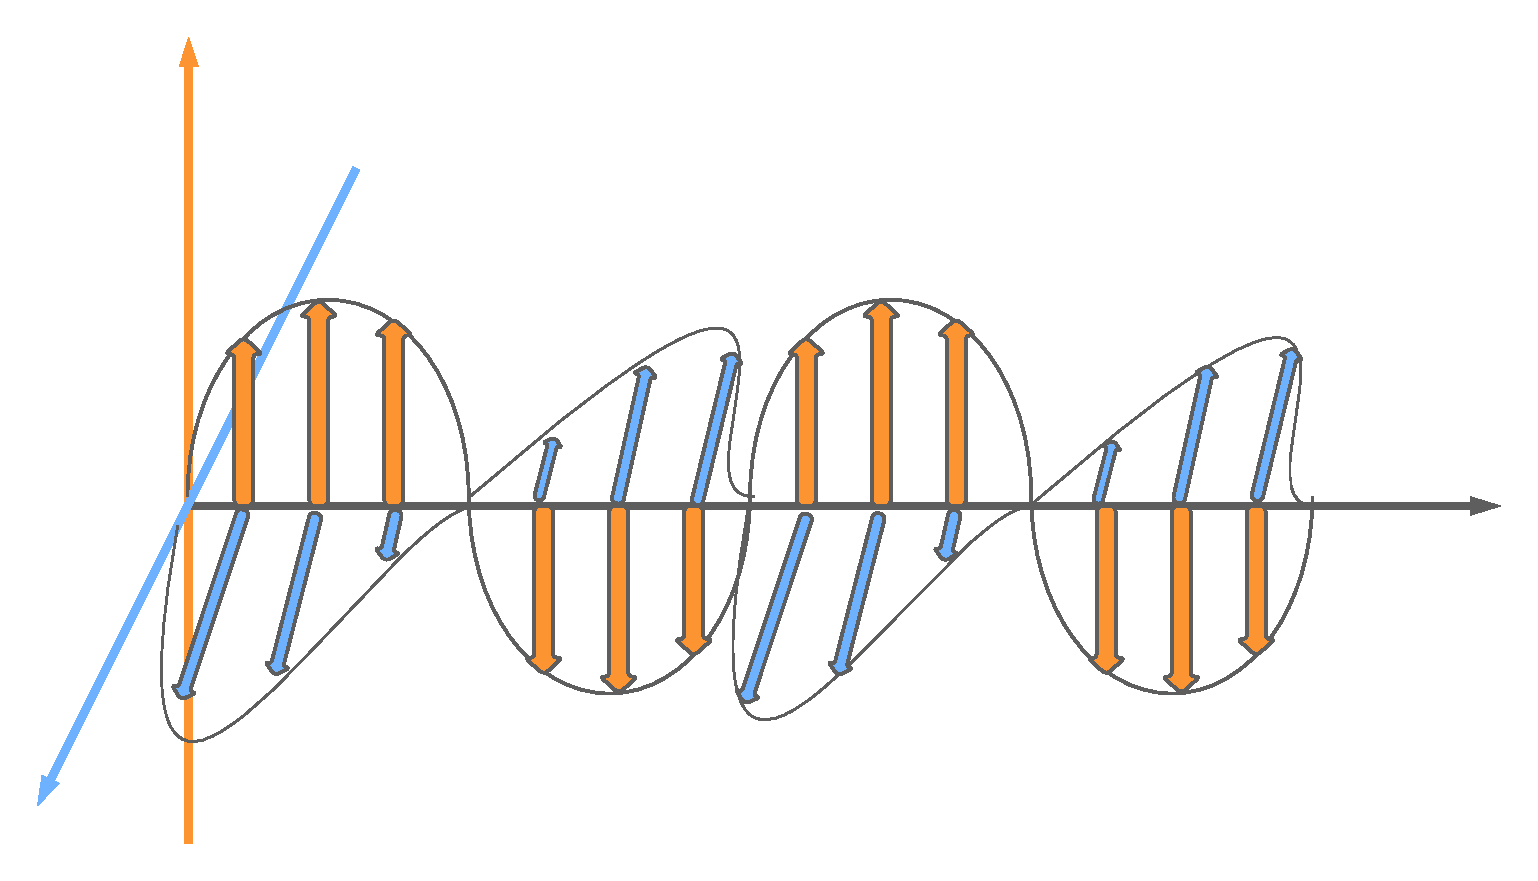
\includegraphics[width=7cm]{./image/wave_propagation.pdf}
  \caption{偏波のイメージ}\label{偏波のイメージ}
  \end{center}
  \end{figure}

 \section{圧縮センシング}
 圧縮センシングとは、対象となる信号をできるだけ少ない観察点数から復元する技術のことである。圧縮技術の多くは、一旦観察信号を
大容量データとして取得した後に圧縮削減するが、圧縮センシングとは観察と圧縮を同時に行うことができ、効率的にデータを取得することが可能である。
\\ 圧縮センシングにおいては「スパース(疎)性」を満たすことが必要である。スパース性とは、ゼロ成分が多く含まれる性質を示し、圧縮センシングでは
ゼロ成分のデータを削減してもキーとなる非ゼロ成分から信号の復元が可能となる。例えば測定データを画像化したものについて考える。理想的な画像では
材質あるいは成分が同じ場合信号強度は等しく、境界面でのみ信号強度が変化すると考えられる。ゆえに境界についての情報が重要となり、画像を境界と
それ以外の情報に分離するような画像変換を行えば、スパース性が高くなり、少ない情報から理想的な画像を再現することができる。


\chapter{提案手法}

\section{図の挿入の仕方}
データは参考文献\cite{rika} にあったものを使った.
この文献\cite{ten}も参考にした。


\chapter{最後に}

結論とか,まとめとか。
最後にいうのもなんだが,ベクトルの書き方。
\begin{itemize}
\item 普通の$\alpha$は\verb|\alpha|で書く。
\item \verb|$\vec{\alpha}$| で $\vec{\alpha}$
\item \verb|\usepackage{bm}| している場合は
\verb|$\bm{\alpha}$| で $\bm{\alpha}$
\item 並べると,$\alpha$, $\vec{\alpha}$, $\bm{\alpha}$
\end{itemize}

\begin{thebibliography}{99}
  \bibitem{rika} 国立天文台編,理科年表 (丸善)
  \bibitem{ten} 天文年鑑,誠文堂新光社。
  \bibitem{phasor}K.Oyama and A.Hirose, "Phasor Quaternion Neural Networks for Singular
  Point Compensation in Polarimetric-Interferometric
  Synthetic Aperture Radar", IEEE Transactions on Geoscience and Remote Sensing, vol. 57, no. 5, May 2019
  \bibitem{human detection}Y.Kim,  Senior Member, IEEE, and T.Moon, "Human Detection and Activity Classification Based
  on Micro-Doppler Signatures Using Deep
  Convolutional Neural Networks", IEEE Geoscience and Remote Sensing Letters,vol. 13,no. 1,January 2016
  \bibitem{imai}R.Imai, Y.Song, R.Natsuaki , Senior Member,and A.Hirose, IEEE Transactions on Geoscience and Remote Sensing, vol. 60, 2022, 
  "Model-Based Homogeneity to Extend Compressed Sensing for Ground Penetrating Radar"
  % \bibitem{jireishuu}https://geology.co.jp/archives/projects/%E5%9C%B0%E4%B8%AD%E3%83%AC%E3%83%BC%E3%83%80%E3%83%BC%E3%81%AE%E6%96%B0%E3%81%9F%E3%81%AA%E4%BA%8B%E4%BE%8B%E9%9B%86%EF%BC%88%E3%82%B1%E3%83%BC%E3%82%B9%E3%82%B9%E3%82%BF%E3%83%87%E3%82%A3%EF%BC%89#case01

  % \bibitem{satou}http://cobalt.cneas.tohoku.ac.jp/users/sato/newpage24.htm#:~:text=%E5%9C%B0%E4%B8%AD%E3%83%AC%E3%83%BC%E3%83%80%E3%81%AF%E9%9B%BB%E7%A3%81%E6%B3%A2,%E3%83%91%E3%83%BC%E3%82%BD%E3%83%8A%E3%83%AB%E3%83%BB%E3%82%B3%E3%83%B3%E3%83%94%E3%83%A5%E3%83%BC%E3%82%BF%E3%81%A7%E8%A8%98%E9%8C%B2%E3%81%99%E3%82%8B%E3%80%82
  % \bibitem{cs}https://www.innervision.co.jp/ressources/pdf/innervision2014/iv201409_061.pdf
 
  \end{thebibliography}
  
  \end{document}